In this section, we describe applied techniques and compare their selected attributed in order to understand how similar different algorithms are.

Applied techniques are described in Table~\ref{table:techniques}. As it is shown eight supervised as well as two unsupervised algorithms wereused.

Since both unsupervised methods (PCI and LSA) reduce the input data to another matrix, the final attributes in the reduced
matrix are not comparable with input data. In the case of applying Ranker search method on any unsupervised evaluators, the ranked attributes will be a sequence from one to the number of attributes. Therefore, we decided to focus more on behavior of supervised methods.

We apply program's algorithm comparison ($-c$ parameter) on the result of eight supervised algorithms. Using provided data, we understand the number of mutual attributes between each pair of algorithms. In order to apply clustering on the methods, a distance matrix is created. To form the matrix, the number of mutual attributes for each pair are subtracted from $50$. The distance matrix of $GTZAN$ dataset is shown in Table~\ref{table:distancematrix}.

In the next step, by using R the methods are clustered based on Hierarchal Clustering algorithm. The clustering results of four datasets are shown in Figure~\ref{fig:clustering}.

Based on the diagrams, the following results can be concluded:
\begin{itemize}
\item ChiSquaredAttribute and InfoGain tend to have very similar results.
\item Besides ChiSquaredAttribute and InfoGain, SymmetricalUncertAttribute is the most similar one to them.
\item ConsistencySubset has always the most different results in comparison to the others.
\item CfsSubset and ReliefFAttribute seems to be related in some cases.
\end{itemize}

\begin{table}[p]
\begin{center}
\begin{tabular}{|c|c|c|c|}
\hline Attribute Evaluator & Search Method & Supervised/Unsupervised & Parameter Name \\
\hline CfsSubset & GreedyStepwise & Supervised & cfs-greedy\\
\hline ChiSquaredAttribute & Ranker & Supervised & chis-ranker\\
\hline ConsistencySubset & BestFirst & Supervised & cons-bestfirst\\
\hline GainRatioAttribute & Ranker & Supervised & gainr-ranker\\
\hline InfoGain & Ranker & Supervised & ig-ranker\\
\hline OneRAttribute & Ranker & Supervised & oner-ranker\\
\hline ReliefFAttribute & Ranker & Supervised & rel-ranker\\
\hline SymmetricalUncertAttribute & Ranker & Supervised & sua-ranker\\
\hline PrincipalComponents & Ranker & Unsupervised & pca-ranker\\
\hline LatentSemanticAnalysis & Ranker & Unsupervised & lsa-ranker\\
\hline
\end{tabular}
\caption{Applied attribute selection techniques}
\label{table:techniques}
\end{center}
\end{table}


\begin{table}[p]
\begin{center}
\begin{tabular}{|c|p{1.3cm}|p{1.3cm}|p{1.3cm}|p{1.3cm}|p{1.3cm}|p{1.3cm}|p{1.3cm}|p{1.3cm}|}
\hline & cfs-greedy & chis-ranker & cons-bestfirst & gainr-ranker & ig-ranker & oner-ranker & rel-ranker & sua-ranker\\
\hline cfs-greedy & 0 & 41 & 46 & 44 & 40 & 39 & 28 & 40\\
\hline chis-ranker & 41 & 0 & 48 & 39 & 9 & 21 & 37 & 9\\
\hline cons-bestfirst & 46 & 48 & 0 & 50 & 48 & 49 & 47 & 49\\
\hline gainr-ranker & 44 & 39 & 50 & 0 & 37 & 34 & 41 & 34\\
\hline ig-ranker & 40 & 9 & 48 & 37 & 0 & 16 & 36 & 4\\
\hline oner-ranker & 39 & 21 & 49 & 34 & 16 & 0 & 37 & 16\\
\hline rel-ranker & 28 & 37 & 47 & 41 & 36 & 37 & 0 & 36\\
\hline sua-ranker & 40 & 9 & 49 & 34 & 4 & 16 & 36 & 0\\
\hline
\end{tabular}
\caption{Applied attribute selection techniques}
\label{table:distancematrix}
\end{center}
\end{table}


\begin{figure}[p]
\begin{center}
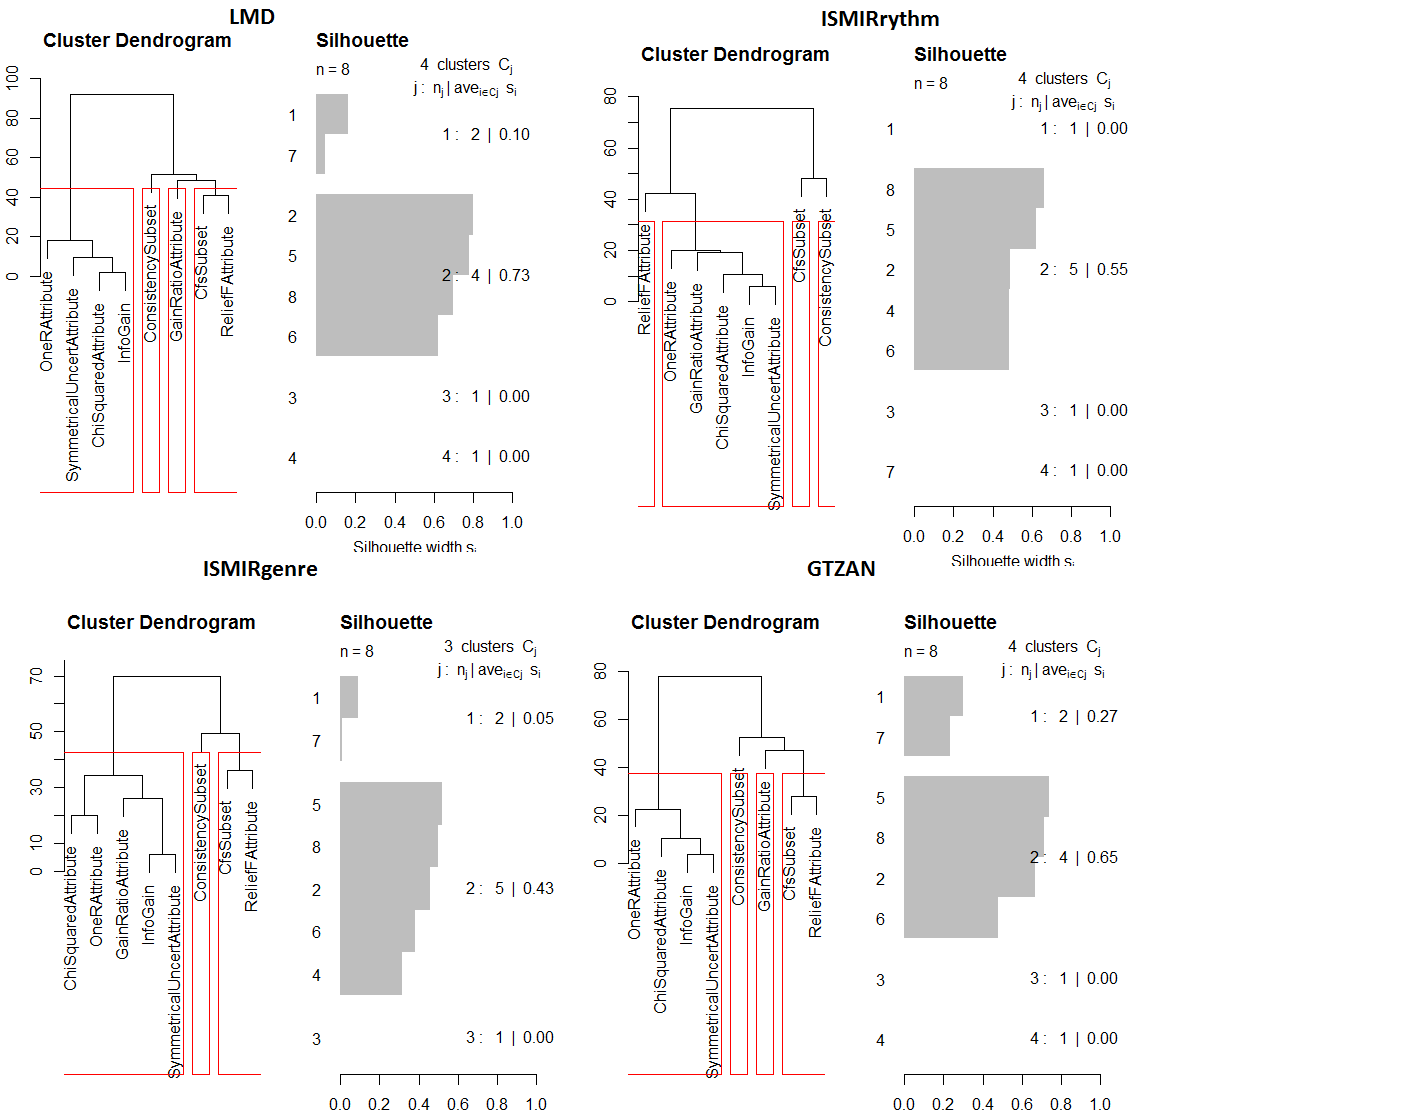
\includegraphics[scale=0.5]{fig/diagram_all.png}
\caption{Attribute selection methods clustering for four datasets
\label{fig:clustering}}
\end{center}
\end{figure}
